%% Template para dissertacaoo/tese na classe UFBAthesis
%% versao 1.0
%% (c) 2005 Paulo G. S. Fonseca
%% (c) 2012 Antonio Terceiro
%% (c) 2014 Christina von Flach
%% www.dcc.ufba.br/~flach/ufbathesis

%% Carrega a classe ufbathesis
%% Opcoes: * Idiomas
%%           pt   - portugues (padrao)
%%           en   - ingles
%%         * Tipo do Texto
%%           bsc  - para monografias de graduacao
%%           msc  - para dissertacoes de mestrado (padrao)
%%           qual - exame de qualificacao de mestrado
%%           prop - exame de qualificacao de doutorado
%%           phd  - para teses de doutorado
%%         * Media
%%           scr  - para versao eletronica (PDF) / consulte o guia do usuario
%%         * Estilo
%%           classic - estilo original a la TAOCP (deprecated) - apesar de deprecated, manter esse.
%%           std     - novo estilo a la CUP (padrao)
%%         * Paginacao
%%           oneside - para impressao em face unica
%%           twoside - para impressao em frente e verso (padrao)

% Aten??o: Manter 'classic' na declaracao abaixo:
\documentclass[en, prop, classic, a4paper]{ufbathesis}

%% Preambulo:
\usepackage[utf8]{inputenc}
\usepackage{graphicx}
\usepackage{lipsum}
\usepackage{hyphenat}
\usepackage[usenames, dvipsnames, table]{xcolor}
\usepackage{booktabs}
\usepackage{pifont}
\usepackage{multirow}
\usepackage{listings} 
\usepackage{colortbl}
\usepackage{xfrac}
\usepackage[FIGTOPCAP]{subfigure}


% Universidade
\university{Universidade Federal da Bahia}

% Endereco (cidade)
\address{Salvador}

% Instituto ou Centro Academico
\institute{Instituto de Matem\'{a}tica}

% Nome da biblioteca - usado na ficha catalografica
\library{Biblioteca Reitor Mac\^{e}do Costa}

% Programa de pos-graduacao
\program{Programa de P\'{o}s-Gradua\c{c}\~{a}o em Ci\^{e}ncia da Computa\c{c}\~{a}o}

% Area de titulacao
\majorfield{Ci\^{e}ncia da Computa\c{c}\~{a}o}

% Titulo da dissertacao ou tese
\title{T\'{\i}tulo da Disserta\c{c}\~{a}o ou Tese}

% Data da defesa
% e.g. \date{19 de fevereiro de 2013}
\date{13 de janeiro de 2014}
% e.g. \defenseyear{2013}
\defenseyear{2014}

% Autor
% e.g. \author{Jose da Silva}
\author{Nome Completo do AUTOR}

% Orientador(a)
% Opcao: [f] - para orientador do sexo feminino
% e.g. \adviser[f]{Profa. Dra. Maria Santos}
\adviser[f]{Nome Completo da ORIENTADORA}

% Orientador(a)
% Opcao: [f] - para orientador do sexo feminino
% e.g. \coadviser{Prof. Dr. Pedro Pedreira}
% Comente se nao ha co-orientador
\coadviser{Nome Completo do CO-ORIENTADOR}

%% Inicio do documento
\begin{document}

\pgcompfrontpage

%% Parte pre-textual
\frontmatter

\pgcomppresentationpage


%%%%%%%%%%%%%%%%%%%%%
% Resumo em Portugues
%%%%%%%%%%%%%%%%%%%%%

\resumo
COLOQUE O RESUMO. Se preferir, crie um arquivo separado e o inclua via comando include.

Para evitar problemas de formato neste template (de uso geral), usamos acentua\c{c}\~{a}o mostrada abaixo. 

\begin{verbatim} 
\c{c} \~{a} \'{a} \^{e} \'{\i}
\end{verbatim} 

N\~{a}o precisa fazer dessa forma, caso use pacotes adequados (latin1, etc.).

% Palavras-chave do resumo em Portugues
\begin{keywords}
PALAVRAS-CHAVE.
\end{keywords}

%%%%%%%%%%%%%%%%%%%
% Resumo em Ingles
%%%%%%%%%%%%%%%%%%%

\abstract
COLOQUE O RESUMO EM INGL\^{E}S. Se preferir, crie um arquivo separado e o inclua via comando include.
% Palavras-chave do resumo em Ingles
\begin{keywords}
PALAVRAS-CHAVE EM INGL\^{E}S.
\end{keywords}

%%%%%%%%%%%%%%%%%%%
% Sumario / Indice
%%%%%%%%%%%%%%%%%%%

% Comente para ocultar
\tableofcontents

% Lista de figuras
% Comente para ocultar
\listoffigures

% Lista de tabelas
% Comente para ocultar
\listoftables

%% Parte textual
\mainmatter

% Eh aconselhavel criar cada capitulo em um arquivo separado, digamos
% "capitulo1.tex", "capitulo2.tex", ... "capituloN.tex" e depois
% inclui-los com:
% \xchapter{Introdução}{ }

O \ac{SAD}, caracteriza-se como uma modalidade de atenção à saúde composta por um conjunto de ações de prevenção, de reabilitação e de tratamento de doenças prestadas em domicílio.
Esse serviço tem se tornado cada vez mais presente de forma a complementar ou substituir a internação hospitalar, pois oferece uma nova forma de atendimento às pessoas com quadro clinico estável que necessitam de cuidados.
Essa modalidade de atendimento permite maior comodidade aos pacientes, aumentando o conforto e facilitando o apoio familiar, além de reduzir os riscos de contaminação hospitalar e a lotação nos hospitais \cite{Kergosien:2009}.
Por outro lado, o \ac{SAD} também possui algum desafios, tais como: a necessidade do deslocamento do profissional de saúde, o planejamento da escada de trabalho dos profissionais de saúde envolvidos, o aumento de custos para a família, nos casos da necessidade de manter equipamentos elétricos ligados, e a eventual estadia do cuidador ou enfermeiro.%\cite{portaL:2017}.   

Na busca da melhor qualidade de vida da população e na redução de custos hospitalares, o \ac{SAD} tem sido bastante incentivado em diversos países. 
No Brasil, esse serviço teve início na década de 1960, porém seu funcionamento foi regulamentado pelo Sistema Único de Saúde (SUS) na década de 90, a partir da lei n. 8.080, de 19 de Setembro de 1990 \cite{Silva:2010}, chegando a Salvador em 2012, através da \ac{FESFSUS}. 

A \ac{FESFSUS} é um órgão público, sem fins lucrativos, que atua em 69 municípios do Estado da Bahia desde a Lei Complementar Estadual n. 29, de 21/12/2007, tendo iniciado suas atividades em 2009, começando a atuar na Bahia a partir de 16 de Abril de 2012. A fundação possui como uma das suas atribuições fornecer atenção domiciliar, de forma gratuita para os moradores da cidade de Salvador e regiões metropolitanas. Atualmente existem 9 bases e 135 pacientes internados em domicílio, e uma equipe de profissionais composta por: dois médicos, um enfermeiro, quatro técnicos de enfermagem, e um fisioterapeuta, contando também com profissionais de apoio, sendo eles: um assistente social, um nutricionista e um fonoaudiólogo.

A \ac{FESFSUS} fornece serviço de atenção domiciliar a pacientes com médio ou alto grau de complexidade, como por exemplo: pacientes com sequelas de acidente vascular cerebral, cardiopatas, portadores de paralisia infantil, politraumatizados, perfurados por armas de fogo e pacientes em tratamento oncológico.

Apesar do \ac{SAD} já existir há bastante tempo e em diversos países, ainda existem alguns desafios, tais como, o planejamento do escalonamento das equipes de atenção domiciliar e do roteamento dos veículos destinados a conduzir as equipes que irão realizar os atendimentos.

O Problema de Escalonamento e Roteamento de Equipes do Serviço de Atenção Domiciliar, conhecido como \ac{HHCP}, tem como objetivo determinar como as visitas podem ser agendadas, e como as equipes devem ser compostas, de forma a fazer o melhor uso das equipes de profissionais de saúde e atender os pacientes da melhor forma possível~\cite{Bertels:2006} e~\cite{Decerle:2016}.

% O Problema de Escalonamento de Equipe de Atenção Domiciliar, conhecido como \ac{HHCSP} tem como objetivo reduzir os custos da equipe do \ac{SAD}, de forma que o atendimento seja realizado de forma eficiente, sem prejudicar a qualidade do serviço, para  que isso seja possível, é necessário levar em consideração o tempo de atendimento $T[e_{i}, l_{i}]$ e o fato do atendimento ser realizado por um grupo de profissionais com diferentes habilidades, pela preferência dos clientes e pelo meio de transporte utilizado~\cite{Bertels:2006}. 

% O  Problema integrado de Escalonamento e Roteamento da Equipe de Atenção Domiciliar, o \ac{HHCRSP}, tem como objetivo construir de forma integrada o roteamento dos veículos da equipe de atendimento domiciliar, assim como, o escalonamento das equipes que serão trasportadas em cada veículo, para que seja possível percorrer todos os locais de visita e atender a um conjunto de pacientes de forma eficiente \cite{Decerle:2016}.  

Foi verificado na literatura estudada a existência de diversas abordagens heurísticas, técnicas baseadas em inteligência artificial, e técnicas baseadas em métodos exatos para solucionar o problema citado.

\section{Motivação e justificativa}

O roteamento e escalonamento das equipes de internação domiciliar ainda é realizado de forma manual em diversos países, inclusive no Brasil, tornando o processo ineficiente e muitas vezes gerando resultados insatisfatórios~\cite{cheng:98},~\cite{bachouch:2010},~\cite{tozlu:2016} e~\cite{cattafi:2012}.
Estima-se que o profissional de atendimento domiciliar passam entre $18\%$ a $26\%$ do tempo de trabalho dentro do veículo realizando translados entre os pontos de atendimento~\cite{holm:2014}.

Acredita-se que a partir da elaboração de escalas de trabalho e de rotas mais eficientes será possível aumentar a cobertura do serviço e sua visibilidade, permitindo a expansão do atendimento a pacientes com baixa complexidade e o aumento da quantidade de atendimentos a pacientes de média ou alta complexidade.  

Observando as dificuldades encontradas por diversos pesquisadores no momento de realizar o roteamento e o escalonamento do Serviço de Atendimento Domiciliar em vários países do mundo, foi idealizada uma proposta de elaborar um estudo de caso do \ac{SAD} em Salvador, e desenvolver uma solução heurística com o objetivo de aumentar o número de atendimentos da equipe de internação domiciliar. 

% \section{Metodologia}
% A metodologia utilizada neste projeto levará em consideração abordagens heurísticas e técnicas de teoria dos grafos, além de um estudo de caso e pesquisa qualitativa e quantitativa.

\section{Hipótese e objetivos}

Nesta seção será apresentada a hipótese do problema, assim como o objetivo geral e específicos.

\textbf{Hipótese}: \emph{É possível desenvolver uma heurística para o \ac{HHCP} aplicando ao caso específico da equipe de atendimento domiciliar FESFSUS, em Salvador, dessa forma, aumentando produtividade da equipe a partir da redução do tempo dentro do veículo, e auxiliando no aumento da eficiência do atendimento domiciliar em Salvador e região metropolitana,  e contribuindo com a expansão da cobertura do programa, possibilitando o atendimento a pacientes com baixa complexidade.}

Este trabalho tem como objetivo principal desenvolver uma solução heurística para maximizar o número de atendimentos da equipe de atenção domiciliar e aplicar ao projeto FESFSUS em Salvador. 

Buscando alcançar o objetivo principal, temos os seguintes objetivos específicos:
\begin{itemize}
\item Analisar o tempo utilizado pela equipe do \ac{SAD} no percurso entre pontos de atendimentos;
\item Analisar o escalonamento das equipes que serão transportadas em cada veículo;
\item Analisar as rotas de veículos elaboradas pela equipe do \ac{SAD};
\item Analisar heurísticas existentes para os problemas de roteamento e escalonamento do \ac{SAD};
\item Propor uma heurística para o problema de escalonamento e roteamento de equipes do \ac{SAD};
%\item Minimizar os custos do \ac{SAD}
%\item Propor uma heurística para o problema integrado de escalonamento e roteamento de veículos do \ac{SAD};
\end{itemize}


\section{Organização do trabalho}
Este trabalho está organizado da seguinte forma: No capítulo 2 serão apresentados os problemas clássicos de roteamento e de escalonamento; no capítulo 3 serão apresentados problemas de roteamento e escalonamento aplicados à área da saúde; no capítulo 4 é apresenta uma revisão sistemática de literatura, descrevendo as heurísticas existentes; e por fim, no capítulo 5 são apresentados os trabalhos relacionados a proposta da dissertação. 
    
% \begin{figure}[ht]
% \begin{center}
% \begin{tikzpicture}[scale=0.4]
% 	%ponto central
% 	\draw node[draw] at (0, 0) {$0$};
% 	\draw node[draw] at (5,5) {$N+1$};

%     %lado direito x
%     \draw[->, red, dotted, thick] (1.5, -0.5) node[below] {$c_{0,1}$} (0.2, 0) -- (2.8, -1.0) ;
%    	\fill[black] (3,-1) circle (2mm) node[above right] {$v_1$};

%     \draw[->, red, dotted, thick] (4.4, -0.6) node[below] {$c_{1,2}$}  (3.2, -1) -- (5.8, 0);
%     \fill[black] (6,0) circle (2mm) node[above right] {$v_2$};

%     \draw[->, red, dotted, thick] (7.4, -0.1) node[below] {$c_{2,3}$}  (6.2, 0) -- (8.8, 0);
%     \fill[black] (9,0) circle (2mm) node[above right] {$v_3$};   
 
%     \draw[->, red, dotted, thick] (10.4, -0.1) node[below] {$c_{3,4}$}  (9.2, 0) -- (11.8, 0);
%     \fill[black] (12,0) circle (2mm) node[above right] {$v_4$};    

%     \draw[->, red, dotted, thick] (10.8, 2) node[below] {$c_{4,5}$}   (11.8, 0.1) -- (9.3, 3);
%     \fill[black] (9.1, 3.1) circle (2mm) node[above right] {$v_5$};    

%    \draw[->, red, dotted, thick] (6.9, 3) node[below] {$c_{5,6}$}   (9, 3.1) -- (6,2 );
%    \fill[black] (5.8, 2) circle (2mm) node[above right] {$v_6$};    

% 	\draw[->, red, dotted, thick]  (4.1, 2.5) node[below] {$c_{6,7}$}  (5.6, 2) -- (3,2 );
%    \fill[black] (2.8, 2) circle (2mm) node[above right] {$v_7$};  
  	
% 	\draw[->, red, dotted, thick]  (3.2, 4) node[below] {$c_{7,N+1}$}   (2.7, 2) -- (4.8,4.6 );
% \end{tikzpicture}
% \end{center}
% \caption{Grafo de pesos?}
% \end{figure}

% \xchapter{Problemas de escalonamento e roteamento}{ }
%Este capítulo apresenta a formulação do problema, as principais definições para o entendimento do mesmo e um resumo de todo o material estudado.}

\presetkeys%
    {todonotes}%
    {inline,backgroundcolor=yellow}{}
% \todo{}


\section{Problema de Alocação de Pessoal}

O Problema de Alocação de Pessoal consiste em atribuir um conjunto de tarefas a um conjunto de pessoas, satisfazendo a um conjunto de restrições \cite{blochiger:2003}.

%O escalonamento de pessoal deve ser realizado de forma que o serviço esteja disponível durante todo o tempo previsto pela organização. Caso o trabalho de uma equipe não interfira ou não dependa do trabalho de outra equipe, então as equipes podem ser escalonadas de forma independente, caso exista alguma relação de dependência, as equipes devem ser escalonadas levando em consideração estas relações \cite{blochiger:2003}.

Sejam $S = \{s_1,s_ 2, ..., s_{|S|}\}$  um conjunto de pessoas e $T = \{t_1, t_2, \ldots, t_{|T|}\}$ e um conjunto de tarefas. Uma solução para o Problema de Alocação de Pessoal pode ser representada por uma matriz $M$, na qual cada célula $m_{f_is_j}$, contém o valor referente a atribuição da tarefa $t_i \in T$ à pessoa $s_j \in S$.

A Tabela \ref{time_table_block}, apresenta um exemplo da alocação de um conjunto de tarefas a um conjunto de pessoas de forma que cada tarefa seja associada a uma pessoa, sendo que o valor $1$ na célula $m_{fs}$ indica que a pessoa $s$ deve executar a tarefa $f$, caso contrário o valor na célula $m_{fs}$ será 0.

\begin{table}[h]
\centering
\caption{Exemplo de alocação de um conjunto de tarefas a um conjunto de pessoas. \label{time_table_block}} 
\begin{tabular}{r|l|l|l|l}
   & $s_1$ & $s_1$ & $s_3$ & $s_4$ \\ \hline
$t_1$ & 0  & 0  & 1  & 0  \\ \hline
$t_2$ & 1  & 0  & 0  & 0  \\ \hline
$t_3$ & 0  & 0  & 0  & 1  \\ \hline
$t_4$ & 0  & 1  & 0  & 0 
\end{tabular}
\end{table}

% O Problema de Alocação de Pessoal pode ser solucionado a partir da variável de decisão $X_{sf}$ , de forma que se o valor alocado for 1, significa que o item foi alocado na tabela e se for 0, significa que o item não foi alocado. 

% Na equação \ref{alocacao_pessoal}, é representada uma solução para uma instância do problema de alocação de pessoal sendo que $X$ denota o conjunto de todas as variáveis de decisão.

%   \begin{equation}
%   \label{alocacao_pessoal}
%   X_{sf} = 
%   \left \{
%   \begin{array}{cc}
%   1, & \mbox{se a pessoa $s$ foi alocada a atividade $f$} \\
%   0, & \mbox{caso contrario} \\
%   \end{array}
%   \right.
%   \end{equation}

%\subsection{Problema de Alocação de Equipe Técnica}
%%UMA ABORDAGEM OTIMIZADA PARA O PROBLEMA DE ALOCAÇÃO DE EQUIPES E ESCALONAMENTO DE TAREFAS PARA A OBTENÇÃO DE CRONOGRAMAS EFICIENTES
%Já no \ac{PAET}, considera-se um conjunto $K=\{k_1, k_2, ..., k_{|K|}\}$ de equipes em que o objetivo consiste em alocar um conjunto de equipes $K$ a um conjunto de tarefas $F$ \cite{Beasley:1996}. Esse problema leva em consideração que todas as equipes são idênticas e estão localizadas no mesmo depósito a partir do qual eles começam e terminam seu dia de trabalho, o número de equipes não pode ser maior do que o número de tarefas que serão executadas e o tempo de execução do conjunto de tarefas não pode exceder o tempo total $T$ \cite{Beasley:1996}.
%
%Para cada tarefa $t\in T$ é associada um custo de execução, uma janela de tempo $[e_t, l_t]$, sendo $e_t$ o tempo de início e $l_t$ o tempo de término, implicando na duração de tempo $l_f - e_f$, o tempo de viagem $\tau$ e o custo $c$ envolvido na viagem da equipe do depósito para a tarefa $f$ \cite{Beasley:1996}.
%
%Sem perda de generalidade, devemos assumir que as tarefas foram numeradas na ordem ascendente. Cada duas tarefas $i$ e $j$, com $j > i$ existe um arco de transição de custo $c_{ij}$, se for possível para a mesma equipe executar a tarefa $i$ e depois executar a tarefa $j$. As tarefas são organizadas de forma a criar um caminho de tarefas que serão executadas pela mesma equipe \cite{Beasley:1996}. 
%
%O objetivo do problema é, encontrar caminhos de custo total mínimo, de modo que cada tarefa seja realizada exatamente uma vez e o tempo de trabalho total envolvido em cada caminho onde, por tempo de trabalho (significamos o tempo decorrido entre a saída do depósito e a chegada de volta ao depósito) não excede o tempo de trabalho disponível \cite{Beasley:1996}.

%Uma modelagem para o \ac{CSP} pode ser representada a partir de um grafo $G = (V, A)$, sendo cada tarefa representadas por um vértice, que estão todos ligados entre si por arestas de transição. Existindo dois depósitos mostrados como $0$ para representar o início do caminho e como $N+1$ para representar o fim do caminho. Devido a dimensão do tempo, não existem ciclos no grafo \cite{Beasley:1996}. 
%checar referência
% O objetivo do problema é encontrar os caminhos disjuntos de $K$ vértices no caminho entre $0$ e $N+1$, de modo que todas as tarefas estejam em um caminho, o tempo de trabalho incluído em cada caminho não exceda o tempo total $\tau$, o custo total dos caminhos seja mínimo.
%checar referência
%como pode ser visto na figura \ref{CSP}.

% \begin{figure}[h]
% \centering
% \caption{Exemplo Crew Scheduling Problem com K = 1}
% \centering
% 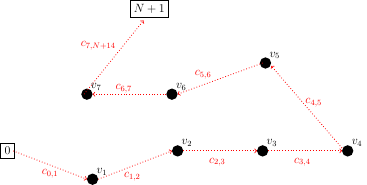
\includegraphics[width=0.8\textwidth]{CSP.png}
% \label{CSP}
% \begin{center}
% Fonte: Elaborada pelo autor
% \end{center}
% \end{figure}

%O objetivo do \ac{CSP} é encontrar todos vértices entre $0$ e $N+1$, tais que todas as tarefas estejam no mesmo caminho, o tempo de trabalho não exceda o tempo total $T$ e o custo total do caminho determinado pelas tarefas executadas seja mínimo. 
% Levando em consideração que cada tarefa pode ser executada apenas uma vez, o custo total associado a cada solução viável é definido pela soma dos custos para realizar cada tarefa $f$, como pode ser visto equação \ref{eqsum}:

% \begin{equation} \label{eqsum}
% 	\sum_{i=1}^{F} c_{f}
%  \end{equation}

% Uma aplicação prática do Crew scheduling problem é o  \textit{Home Care Crew Scheduling Problem}, é um problema no qual uma equipe do \ac{HHCSP} realiza uma série de visitas às casas dos pacientes \cite{rasmussenm:2012}.
%e deve ser encontrado uma solução ótima de forma que todas as visitas sejam feitas no menor tempo possível sem prejudicar a qualidade do atendimento. Este problema foi classificado pelo autor como NP-completo, pois foi verificado a viabilidade em reduzi-lo ao problema do caixeiro viajante, dessa forma, para resolver o problema o autor desenvolveu um algoritmo \textit{branch-and-price}. 

% Uma instância qualquer do problema geral de alocação de equipes pode ser solucionada a partir da variável de decisão $X_{fk}$, tais que, o valor $1$ é associado a uma ligação entre dois vértices, e o valor $0$ determina que não existe uma ligação entre os vértices. Como podemos ver na equação \ref{eqcsp}, que recebe o valor $1$ caso a tarefa $f$ seja associada a equipe $k$ e o valor $0$ caso contrário.

%   \begin{equation} \label{eqcsp}
%   X_{fk} = 
%   \left \{
%   \begin{array}{cc}
%   1, & \mbox{se existe a tarefa $f$ foi alocada a equipe $k$}  \\
%   0, & \mbox{caso contrario} \\
%   \end{array}
%   \right.
%   \end{equation}
  
% A tabela \ref{tarefa_equipe} ilustra um exemplo da solução para o problema de alocação de equipes, no qual cada tarefa $k$ é associada a uma equipe $e_{i}$. 

% \begin{table}[h]
% \centering
% \caption{Tabela: Tarefa X equipes}
% \label{tarefa_equipe}
% \begin{tabular}{l|l|l|l|l}
%    & k1 & k2 & k3 & k4 \\ \hline
% e1 & 0  & 1  & 0  & 0  \\ \hline
% e2 & 0  & 0  & 0  & 1  \\ \hline
% e3 & 0  & 0  & 1  & 0  \\ \hline
% e4 & 1  & 0  & 0  & 0 
% \end{tabular}
% \end{table}

% \subsection{Problema de Alocação de Recursos}

% O problema geral de alocação de recursos consiste em conjunto $R = \{1, 2, ..., r\}$ de recursos que serão escalonados; um custo $c_{r}$ representando o tempo que cada recurso permanecerá alocado, e  um conjunto de processadores  $\Omega = \{1,2, ..., \omega \}$ \cite{ullman:1975}. 
% Como podemos ver na tabela \ref{alocacao_recurso}, no qual o valor é $1$ quando o recurso é alocado no processador $p$ e $0$ quando não é alocado no processador $p$. O objetivo deste problema é executar $k$ recursos dentro do tempo $t$.

% \begin{table}[h]
% \centering
% \caption{Tabela Recurso X Processador \label{alocacao_recurso}}
% \begin{tabular}{l|l|l|l|l}
%    & $\omega1$ & $\omega2$ & $\omega3$ & $\omega4$ \\ \hline
% r1 & 0  & 1  & 0  & 0  \\ \hline
% r2 & 0  & 0  & 0  & 1  \\ \hline
% r3 & 0  & 0  & 1  & 0  \\ \hline
% r4 & 1  & 0  & 0  & 0 
% \end{tabular}
% \end{table}

% O problema de alocação de recursos pode ser solucionado a partir de uma variável de de decisão $X_{r\omega}$, sendo o valor $1$ é atribuído caso o recurso seja associado ao processador, e $0$ se não foi atribuído, como podemos ver na equação \ref{alocacao_recurso}.

%   \begin{equation}
%   \label{alocacao_recurso}
%   X_{rp} = 
%   \left \{
%   \begin{array}{cc}
%   1, & \mbox{ se o recurso $r$ foi alocado ao processador $p$}  \\
%   0, & \mbox{caso contrario} \\
%   \end{array}
%   \right.
%   \end{equation}

\section{Problema do caixeiro viajante}

%O \ac{PCV} é um problema de otimização combinatória no qual, dado um conjunto de cidades e as distâncias entre elas, o objetivo é encontrar o caminho de custo mínimo que passe por cada cidade exatamente uma vez \cite{goyal:2010}.

Seja um grafo $G = (V,A)$, no qual $V$ é um conjunto de vértices e $A$ é um conjunto de arestas, e seja $\tau:V\times V \rightarrow \mathds{R}$ uma função que associa cada par de vértices a uma distância. O \ac{PCV} consiste em determinar um circuito de tamanho mínimo que passa por cada vértice apenas uma vez. Esse circuito é conhecido como um circuito Hamiltoniano \cite{laporte:1992}.

São estudadas diversas variações do \ac{PCV} existindo várias aplicações práticas para o problema, porém neste trabalho serão descritos o \ac{PMCV} e do \ac{PCVJT}. O \ac{PMCV} é uma generalização do \ac{PCV} em que considera um conjunto de caixeiros viajantes, e tem como objetivo determinar, para cada caixeiro, uma rota de custo mínimo onde cada cidade deve ser visitada uma única vez por um único caixeiro viajante~\cite{meng:2012}.  Já no \ac{PCVJT} cada cliente possui um tempo de serviço delimitado por uma janela de tempo definindo o tempo de início e fim do atendimento. As visitas devem ser realizadas respeitando a janela de tempo. O \ac{PCVJT} tem como objetivo encontrar um circuito de custo mínimo, começando e terminando no mesmo depósito e visitando a um conjunto de clientes uma única vez respeitando a janela de tempo de visitação. \cite{urrutia:2010}.

<<<<<<< HEAD
%Seja grafo $G = (V,A,\tau)$, no qual $V = \{v_1, v_2, ..., v_{|V|}\}$ é um conjunto de vértice onde cada um dos seus elementos está associado a uma cidade, e $A = \{ v_i,v_j: v_i,v_j \in V, i \neq j \}$ é uma aresta com uma matriz custo não negativo $C = \{c_{ij}: o \ peso \ de \ (v_i,v_j)\}$. A distância entre $v_i$ e $v_j$ é denotada por $w_{ij}$. 
=======
Seja grafo $G = (V,A,C)$, no qual $V = \{v_1, v_2, ..., v_{|V|}\}$ é um conjunto de vértice onde cada um dos seus elementos está associado a uma cidade, e $A = \{(v_i,v_j): v_i,v_j \in V, i \neq j \}$ é um conjunto de arestas com uma matriz custo não negativo $C = \{c_{ij}: o \ peso \ de \ (v_i,v_j)\}$. A distância entre $v_i$ e $v_j$ é denotada por $c_{ij}$. O \ac{PMCV}, tem como objetivo determinar um conjunto de rotas de custo mínimo que serão percorridas por um conjunto de Caixeiros Viajantes \cite{meng:2012}. 
>>>>>>> bf11a0f8ae334fbc15fd76daf22b0b0f7918b723

%Seja $G=(V,A)$ um grafo, onde $V = \{v_0, v_1, ..., v_{|V|} \}$ é um conjunto de nós, sendo que o nó $0$ representa o depósito e $A = \{ (i,j): i,j \in V, i \neq j \}$ é um conjunto de arestas. O custo de viajar de $i$ para $j$ é representado por $c_{ij}$. Cada cliente $i$ possui uma janela de tempo associada $[e_i, l_i]$, na qual $e_i$ e $l_i$representam o tempo de início e final do atendimento respectivamente. O \ac{PCVJT} consiste em encontrar um circuito hamiltoniano a partir do depósito que satisfaça todas as janelas de tempo e minimize a distância total percorrida\cite{urrutia:2010}.

\section{Problema de roteamento de veículos}

No \ac{PRV} tem como objetivo encontrar uma rota com custo mínimo de modo que seja cumprida a demanda dos clientes. A rota começa e termina no depósito e cada local é visitado apenas uma vez. Cada local é visitado uma vez, e cada veículo possui uma capacidade limitada \cite{gold:2008}.

Seja um conjunto de clientes $Q = \{q_1, q_2, ..., q_{|Q|}\}$, que residem em locais $W = \{w_0, w_1, w_2, ..., w_{|W|}\}$ diferentes. Cada par de locais $(i,j)$, onde  $i,j \in W$ e $i \neq j$, é associado a um tempo de translado $\tau$ e uma distância $u_{ij}$. O depósito, local de onde os veículos partem e retornam, é denotado por $w_0$.
Os clientes são atendidos a partir de um depósito com uma frota  homogênea $Z = \{1, 2, ..., z_{|Z|}\}$ de veículos com capacidade uniforme $y$~\cite{gold:2008}.

O Problema de Roteamento de Veículo com Janela de tempo, o \ac{VRPTW}, assim como o \ac{VRP}, consiste em encontrar um conjunto de rotas com custo mínimo, porém cada cliente $q$ possui uma janela de tempo $[e_{q}, l_{q}]$, sendo $e_{q}$ o tempo de início do atendimento e $l_{q}$ o tempo do fim do atendimento~\cite{gold:2008}.
% ...
% \include{capituloN}
%
% Importante: 
% Use \xchapter{}{} ao inves de \chapter{}; se n?o quiser colocar texto antes do inicio do capitulo, use \xchapter{texto}{}.

\xchapter{Introdu\c{c}\~{a}o}{Este eh o primeiro cap\'{\i}tulo, onde eu conto toda a historia deste trabalho, o problema, a solu\c{c}\~{a}o, etc.}

\section{Se\c{c}\~{a}o}
\lipsum

\subsection{Uma Subse\c{c}\~{a}o}

Texto.

\subsection{Outra Subse\c{c}\~{a}o}

Texto.

\section{Outra Se\c{c}\~{a}o}
\lipsum

\xchapter{Revis\~{a}o Bibliogr\'{a}fica}{Neste cap\'{\i}tulo eu apresento todo o material que eu estudei durante a elabora\c{c}\~{a}o do trabalho.}

\lipsum

Livro \cite{demeyer2008} e  livro \cite{raymond1999}.

\xchapter{Exemplos}{} %sem preambulo

A numera\c{c}\~{a}o de figuras \'{e} sequencial, dentro do cap\'{\i}tulo. Ver Figura \ref{default-regular1} e Figura \ref{default-regular2}.

A numera\c{c}\~{a}o de tabelaas \'{e} sequencial, dentro do cap\'{\i}tulo. Ver Tabela \ref{default-table1} e Tabela \ref{default-table2}.


\section{Exemplos de Figura}

\begin{figure}[htbp]
\begin{center}
  
\includegraphics[scale=0.5]{ufba.eps}
\caption{Bras\~{a}o da UFBA - Menor.}
\label{default-regular1}
\end{center}
\end{figure}

\begin{figure}[htbp]
\begin{center}
  
\includegraphics[scale=0.75]{ufba.eps}
\caption{Bras\~{a}o da UFBA - Maior.}
\label{default-regular2}
\end{center}
\end{figure}

\lipsum

\section{Exemplos de Tabela}
\subsection{Uma Tabela}
\begin{table}[htbp]
\caption{Uma tabela com 3 linhas e 2 colunas.}
\begin{center}
\begin{tabular}{|c|c|} 
\hline
elemento 11 & elemento 12 \\ \hline
elemento 21 & elemento 22 \\ \hline
elemento 31 & elemento 32 \\
\hline
\end{tabular}
\end{center}
\label{default-table1}
\end{table}%

\lipsum

\begin{table}[htbp]
\caption{Uma tabela com 3 linhas e 3 colunas.}
\begin{center}
\begin{tabular}{|l|c|c|} 
\hline
elemento 11 & elemento 12 & elemento 13\\ \hline
elemento 21 & elemento 22 & elemento 23\\ \hline
elemento 31 & elemento 32 & elemento 33\\
\hline
\end{tabular}
\end{center}
\label{default-table2}
\end{table}%

\xchapter{Outro cap\'{\i}tulo}{} %sem preambulo
\lipsum


%% Parte pos-textual
\backmatter

% Bibliografia
% ? aconselh?vel utilizar o BibTeX a partir de um arquivo, digamos "biblio.bib".
% Para ajuda na cria??o do arquivo .bib e utiliza??o do BibTeX, recorra ao
% BibTeXpress em www.cin.ufpe.br/~paguso/bibtexpress
\bibliographystyle{abntex2-alf}
\bibliography{biblio}

% Apendices
% Comente se naoo houver apendices
\appendix

\xchapter{Exemplo de Ap\^endice}{} %sem preambulo
\lipsum
% Eh aconselhavel criar cada apendice em um arquivo separado, digamos
% "apendice1.tex", "apendice.tex", ... "apendiceM.tex" e depois
% inclui--los com:
% \include{apendice1}
% \include{apendice2}
% ...
% \include{apendiceM}

%% Fim do documento
\end{document}
%------------------------------------------------------------------------------------------%
